\providecommand{\main}{../../../..}
\documentclass[\main/dresen_thesis.tex]{subfiles}
  \renewcommand{\thisPath}{\main/chapters/monolayers/structureModel/verticalStructure}

\begin{document}
  \label{sec:monolayers:structure:verticalModel}
  \begin{figure}[tb]
    \centering
    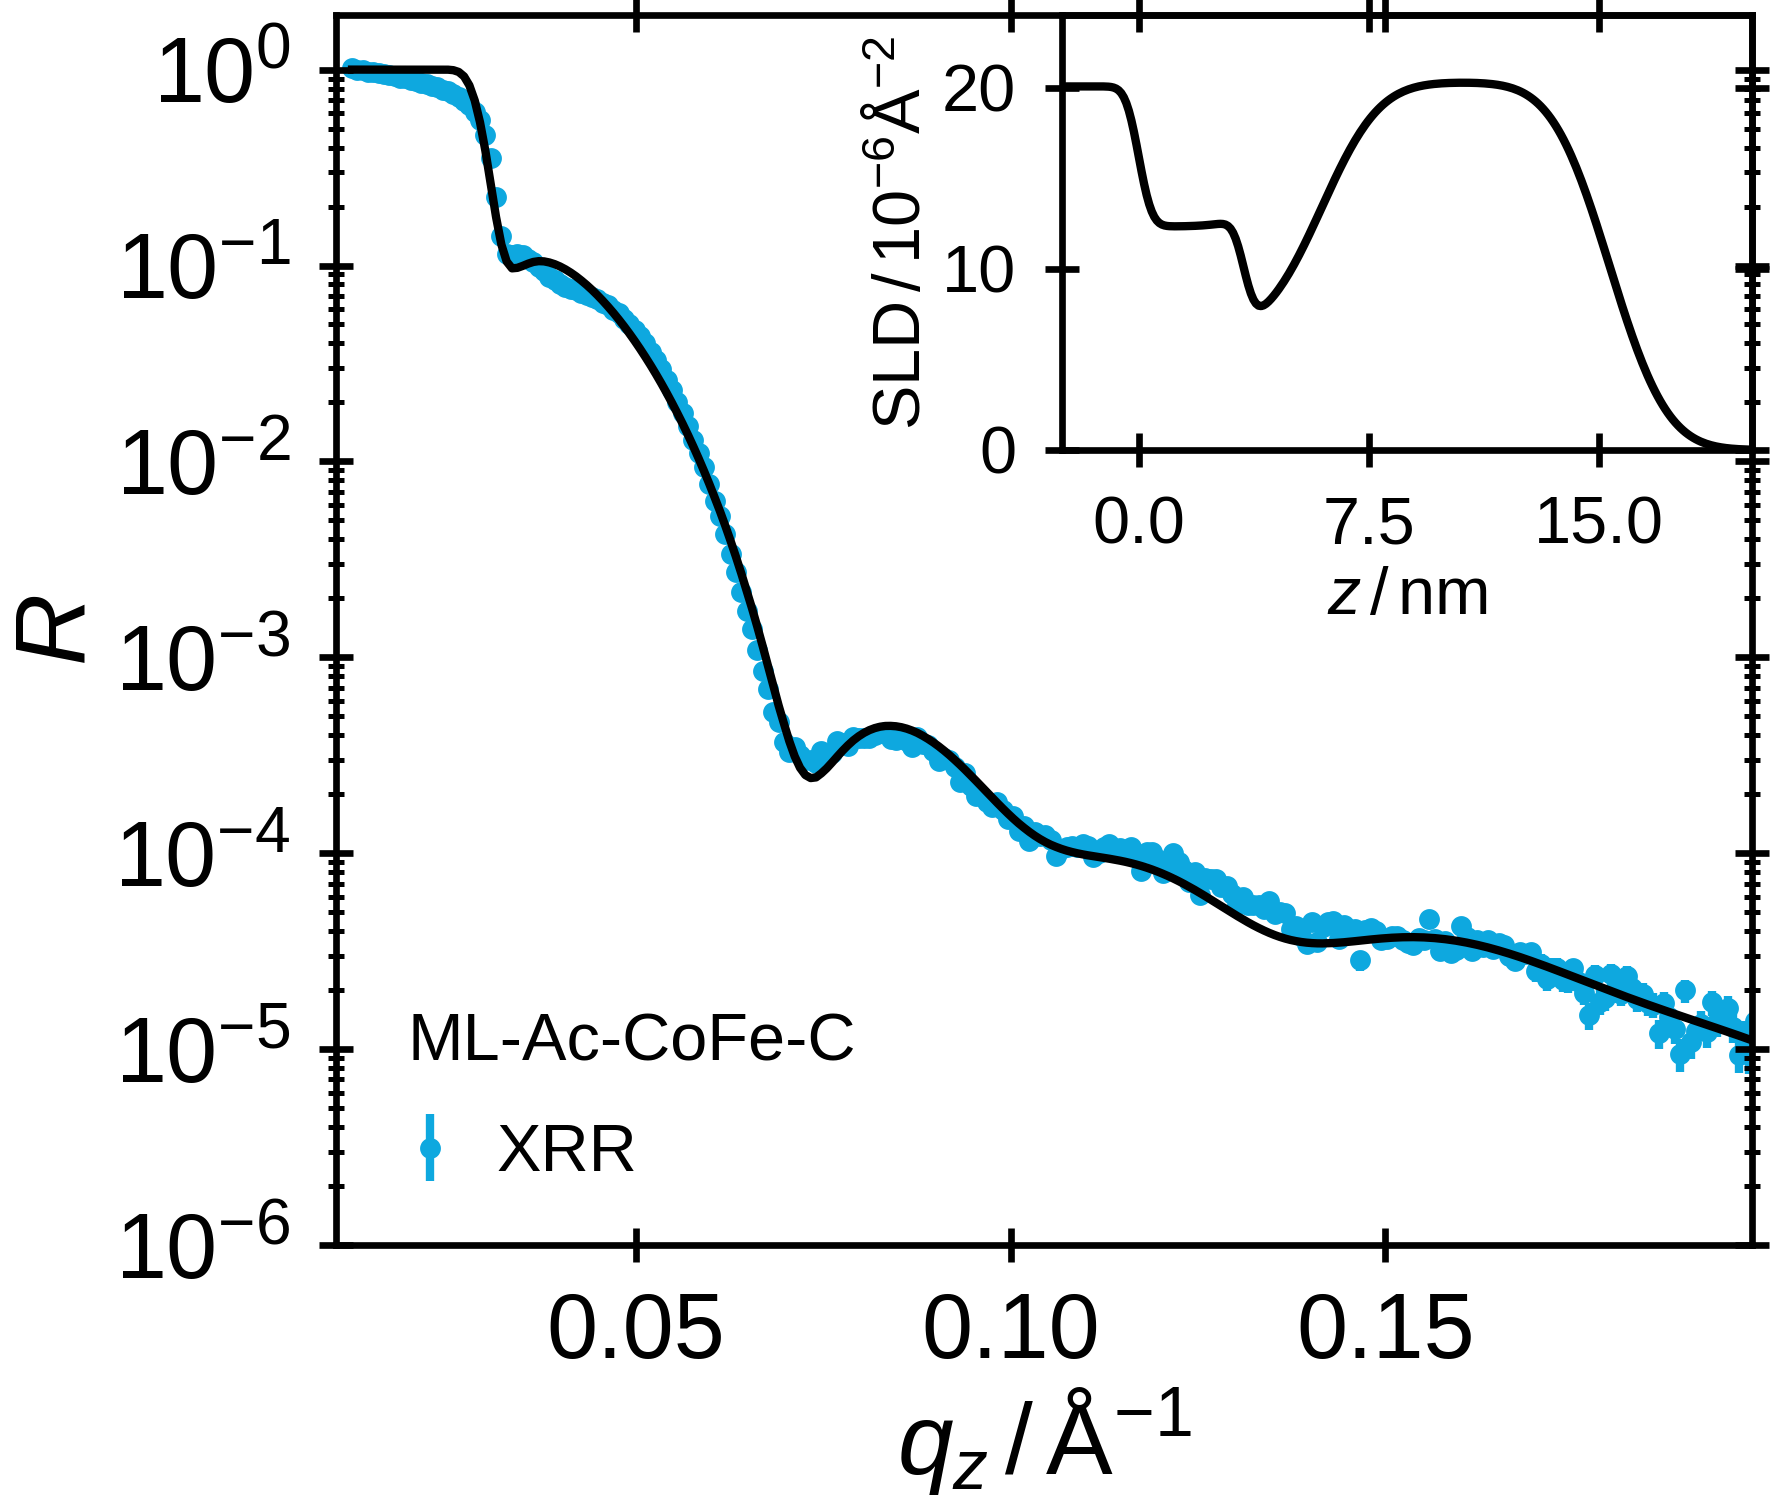
\includegraphics{monolayers_VerticalStructure_ML_Ac-CoFe-C_WithSpacer_XRR}
    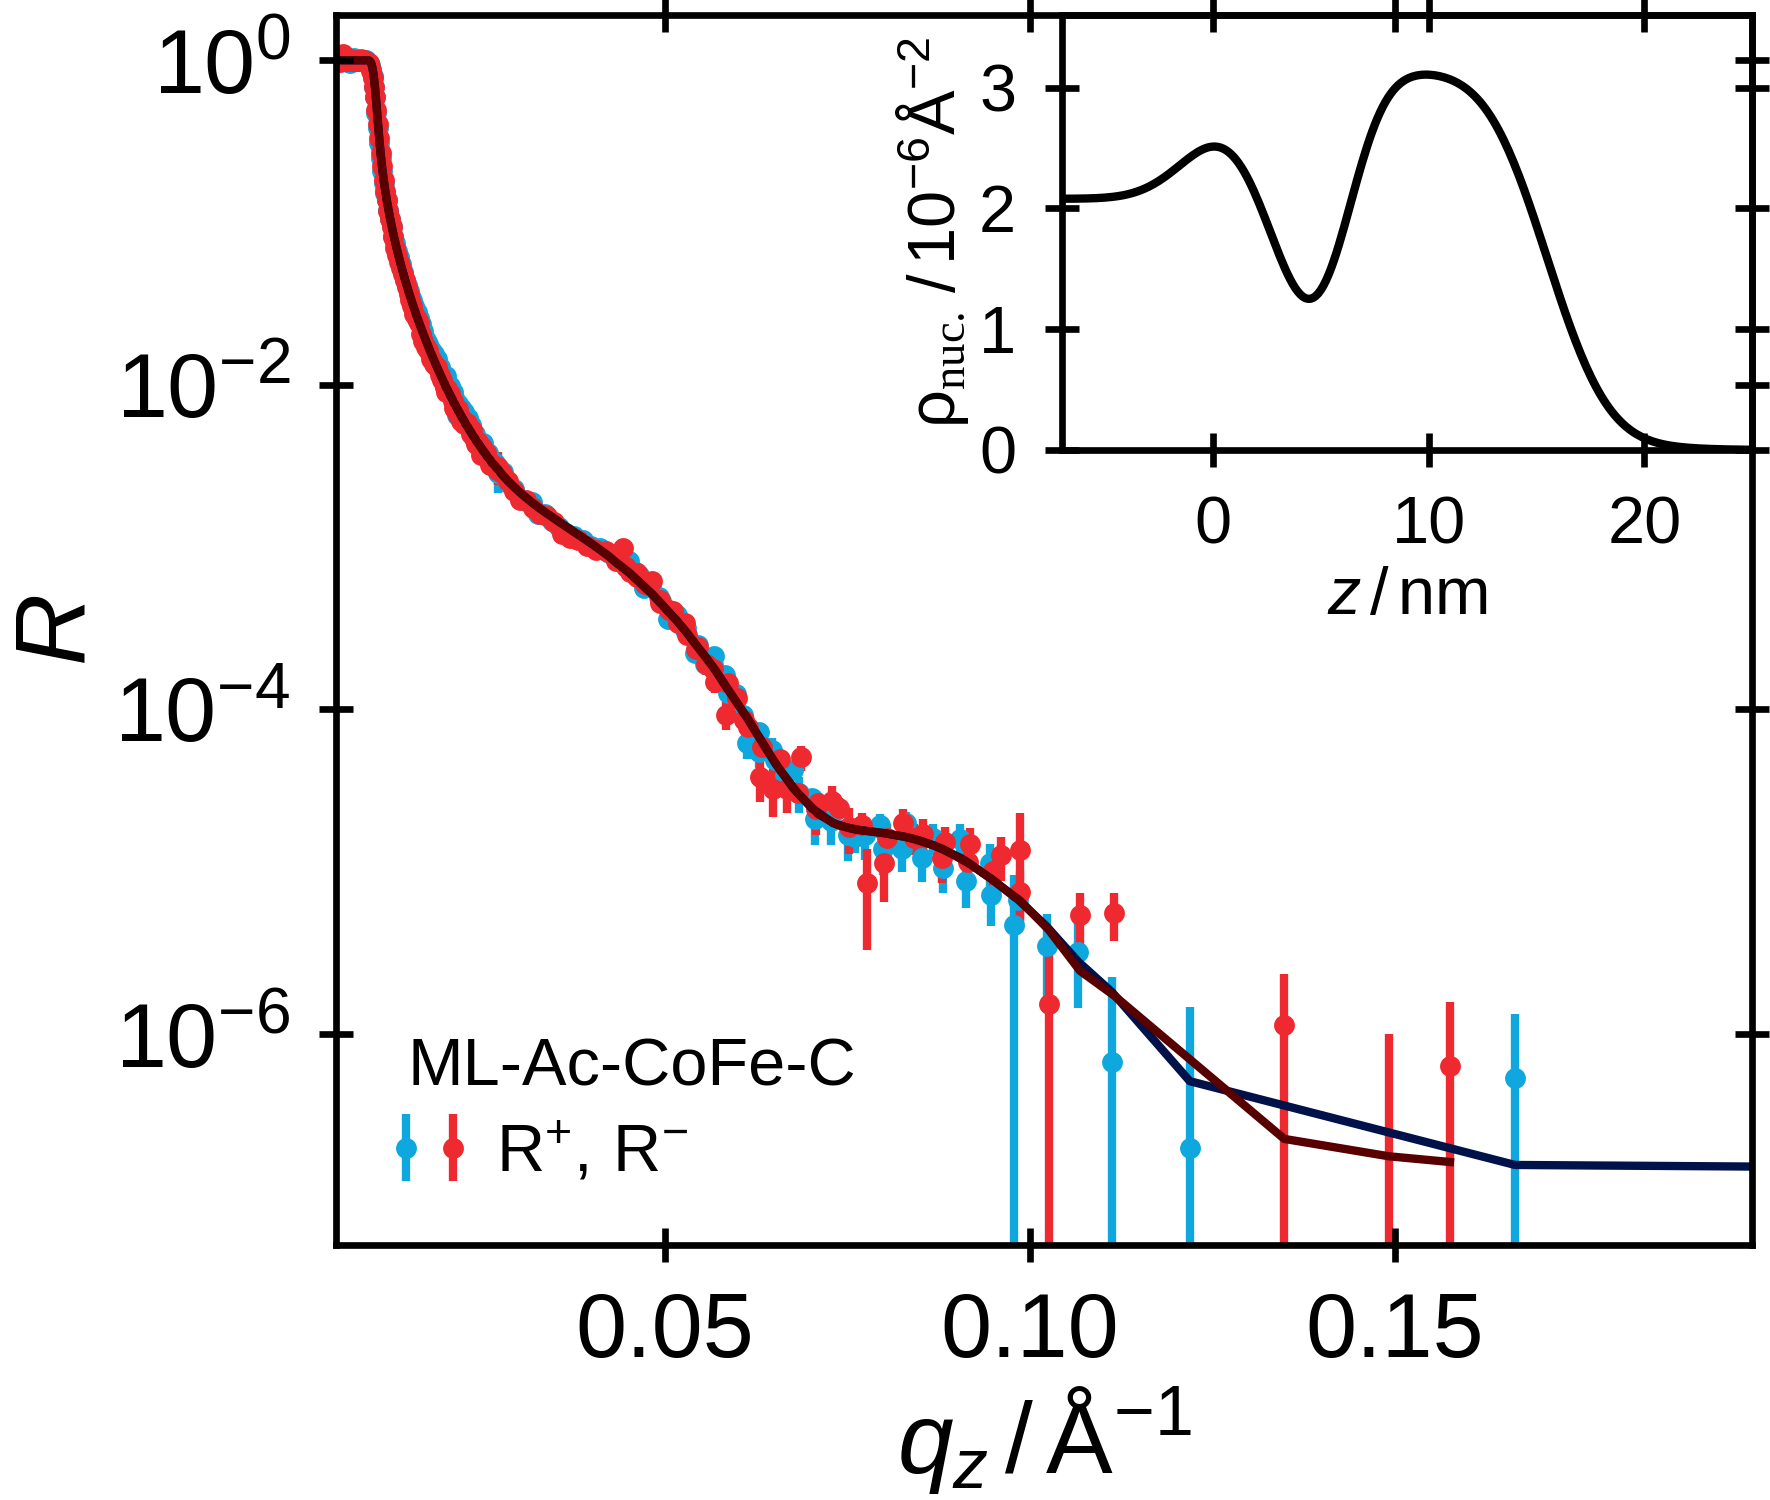
\includegraphics{monolayers_VerticalStructure_ML_Ac-CoFe-C_WithSpacer_NR}
    \caption{\label{fig:monolayers:structure:XRR:ML-Ac-CoFe-C-WithSpacer}X-Ray (left) and neutron
    reflectometry of ML-Ac-CoFe-C described by the model presented in \reffig{fig:monolayers:structure:verticalModel}. The refined scattering length density is presented in the inset.}
  \end{figure}

  X-ray reflectometry is used to yield information on the average electron density distribution with respect to the vertical axis, whereas neutron reflectometry is used to yield information on the nuclear structure and to study subsequently the spin density of the monolayer by discussing data from polarized neutrons.
  \reffig{fig:monolayers:structure:XRR:ML-Ac-CoFe-C-WithSpacer} shows both XRR and NR data measured for ML-Ac-CoFe-C.
  The X-ray data has been measured at ambient conditions on a Bruker D8 Advance (\refsec{ch:instruments:laboratoryInstruments:xrr}) and the neutron reflectivity was measured at D17 in the Institute Laue-Langevin (\refsec{ch:lss:d17}) at $5 \unit{K}$ after zero-field cooling.
  The samples have been fit to the scattering length density profile of oleic acid-ligated nanocubes on a silicon
  substrate with a silicon dioxide intermediate spacer layer.
  The roughness and thickness of the separate layers are refined independently to obtain a close agreement between the calculated and observed reflectivity, where the best results are shown in the insets of \reffig{fig:monolayers:structure:XRR:ML-Ac-CoFe-C-WithSpacer}, with the parameters tabulated in \reftab{tab:monolayers:structure:ML-Ac-CoFe-C-WithSpacer}.

  \begin{table}[!htbp]
    \centering
    \caption{\label{tab:monolayers:structure:ML-Ac-CoFe-C-WithSpacer}Refined parameters from X-ray and neutron reflectometry of ML-Ac-CoFe-C used for the scattering length density profile shown in the insets of \reffig{fig:monolayers:structure:XRR:ML-Ac-CoFe-C-WithSpacer}. The parameter $\eta$ is the packing density factor, $d_{\ch{SiO2}}$ the thickness of the silicon dioxide layer, $d_{\mathrm{OA}}$ the oleic acid layer thickness, $\sigma$ the respective interfacial roughness parameters, $\Delta \lambda / \lambda$ the instrumental wavelength spread and $I_\mathrm{bg}$ a constant background parameter. The nanocube size $a$ is set to the value obtained from SAXS (\refsec{sec:monolayers:nanoparticle:sas}) and the interparticle distance $a_\mathrm{p-p}$ is determined from $\eta$ by \refeq{eq:monolayers:characterization:particleSpacing}.}
    \begin{tabular}{l | c | c}
      \hline
      ML-Ac-CoFe-C & \textbf{XRR} & \textbf{NR}\\
      \hline
      $\eta \, /\, \%$                               & $55.3(8)$  & $50.6(5)$  \\
      $d_{\ch{SiO2}} \, / \unit{nm}$                 & $5.2(5)$   & $2.4(3)$  \\
      $d_{\mathrm{OA, lower}} \, / \unit{nm}$        & $4.5(3)$   & $3.7(3)$  \\
      $d_{\mathrm{OA, upper}} \, / \unit{nm}$        & $3.2(1)$   & $-$  \\
      $\sigma_{\ch{Si}/\ch{SiO2}} \, / \unit{nm}$    & $1.2(3)$   & $2.0(2)$  \\
      $\sigma_{\ch{SiO2}/\mathrm{OA}}\, / \unit{nm}$ & $3.3(4)$   & $2.4(3)$  \\
      $\sigma_\mathrm{OA/NC} \, / \unit{nm}$         & $1.8(1)$   & $1.5(1)$  \\
      $\sigma_\mathrm{NC/OA} \, / \unit{nm}$         & $0.5(1)$   & $2.2(1)$  \\
      $\sigma_\mathrm{OA/air} \, / \unit{nm}$        & $0.9(1)$   & $-$  \\
      $\Delta \lambda / \lambda \, / \unit{\%}$      & $5.0 $     & from inst. spec.\\
      $I_\mathrm{bg}\,/\unit{10^{-6}}$               & $0.95(3)$  & $0.1(1)$\\
      \hline
      $a \, / \unit{nm}$                             & \multicolumn{2}{c}{$9.38$} \\
      \hline
      $a_\mathrm{p-p} \, / \unit{nm}$                & $14.3(2)$     & $13.3(1)$ \\
      \hline
    \end{tabular}
  \end{table}

  The X-ray and neutron reflectivity can both be well described by the simple model of a monolayer and the obtained results are in good agreement.
  The packing fraction of the nanocubes corresponds to a particle spacing of $13.3 - 14.3 \unit{nm}$, which is approximately two oleic acid chain lengths added on top of the nanocube edge length of $9.38 \unit{nm}$ and therefore corresponds to the intuitive expectation.
  For the silicon dioxide spacer thickness, a value of $5.2(5) \unit{nm}$ is estimated with  XRR, whereas $2.4(3) \unit{nm}$ is estimated by NR.
  This can be led back to the small contrast of silicon dioxide and silicon for X-rays, from which a proper estimate of the thickness is more difficult to achieve.
  The lower oleic acid layer has in both cases a thickness of approximately $4 \unit{nm}$, which is thicker than expected from the particle coating alone, and suggests that oleic acid remnants from the drop casting process remain between silicon dioxide and the nanoparticle layer.
  For the upper oleic acid layer, the contrast between oleic acid and air is too low to resolve it, whereas for X-rays again a value that is slightly larger than the surfactant thickness is observed.
  The observed roughness of the sample is in a reasonable order of $1 - 3 \unit{nm}$ for the layers, which can be interpret from the waviness of the sample \eg due to the particle size distribution.

  \begin{figure}[tb]
    \centering
    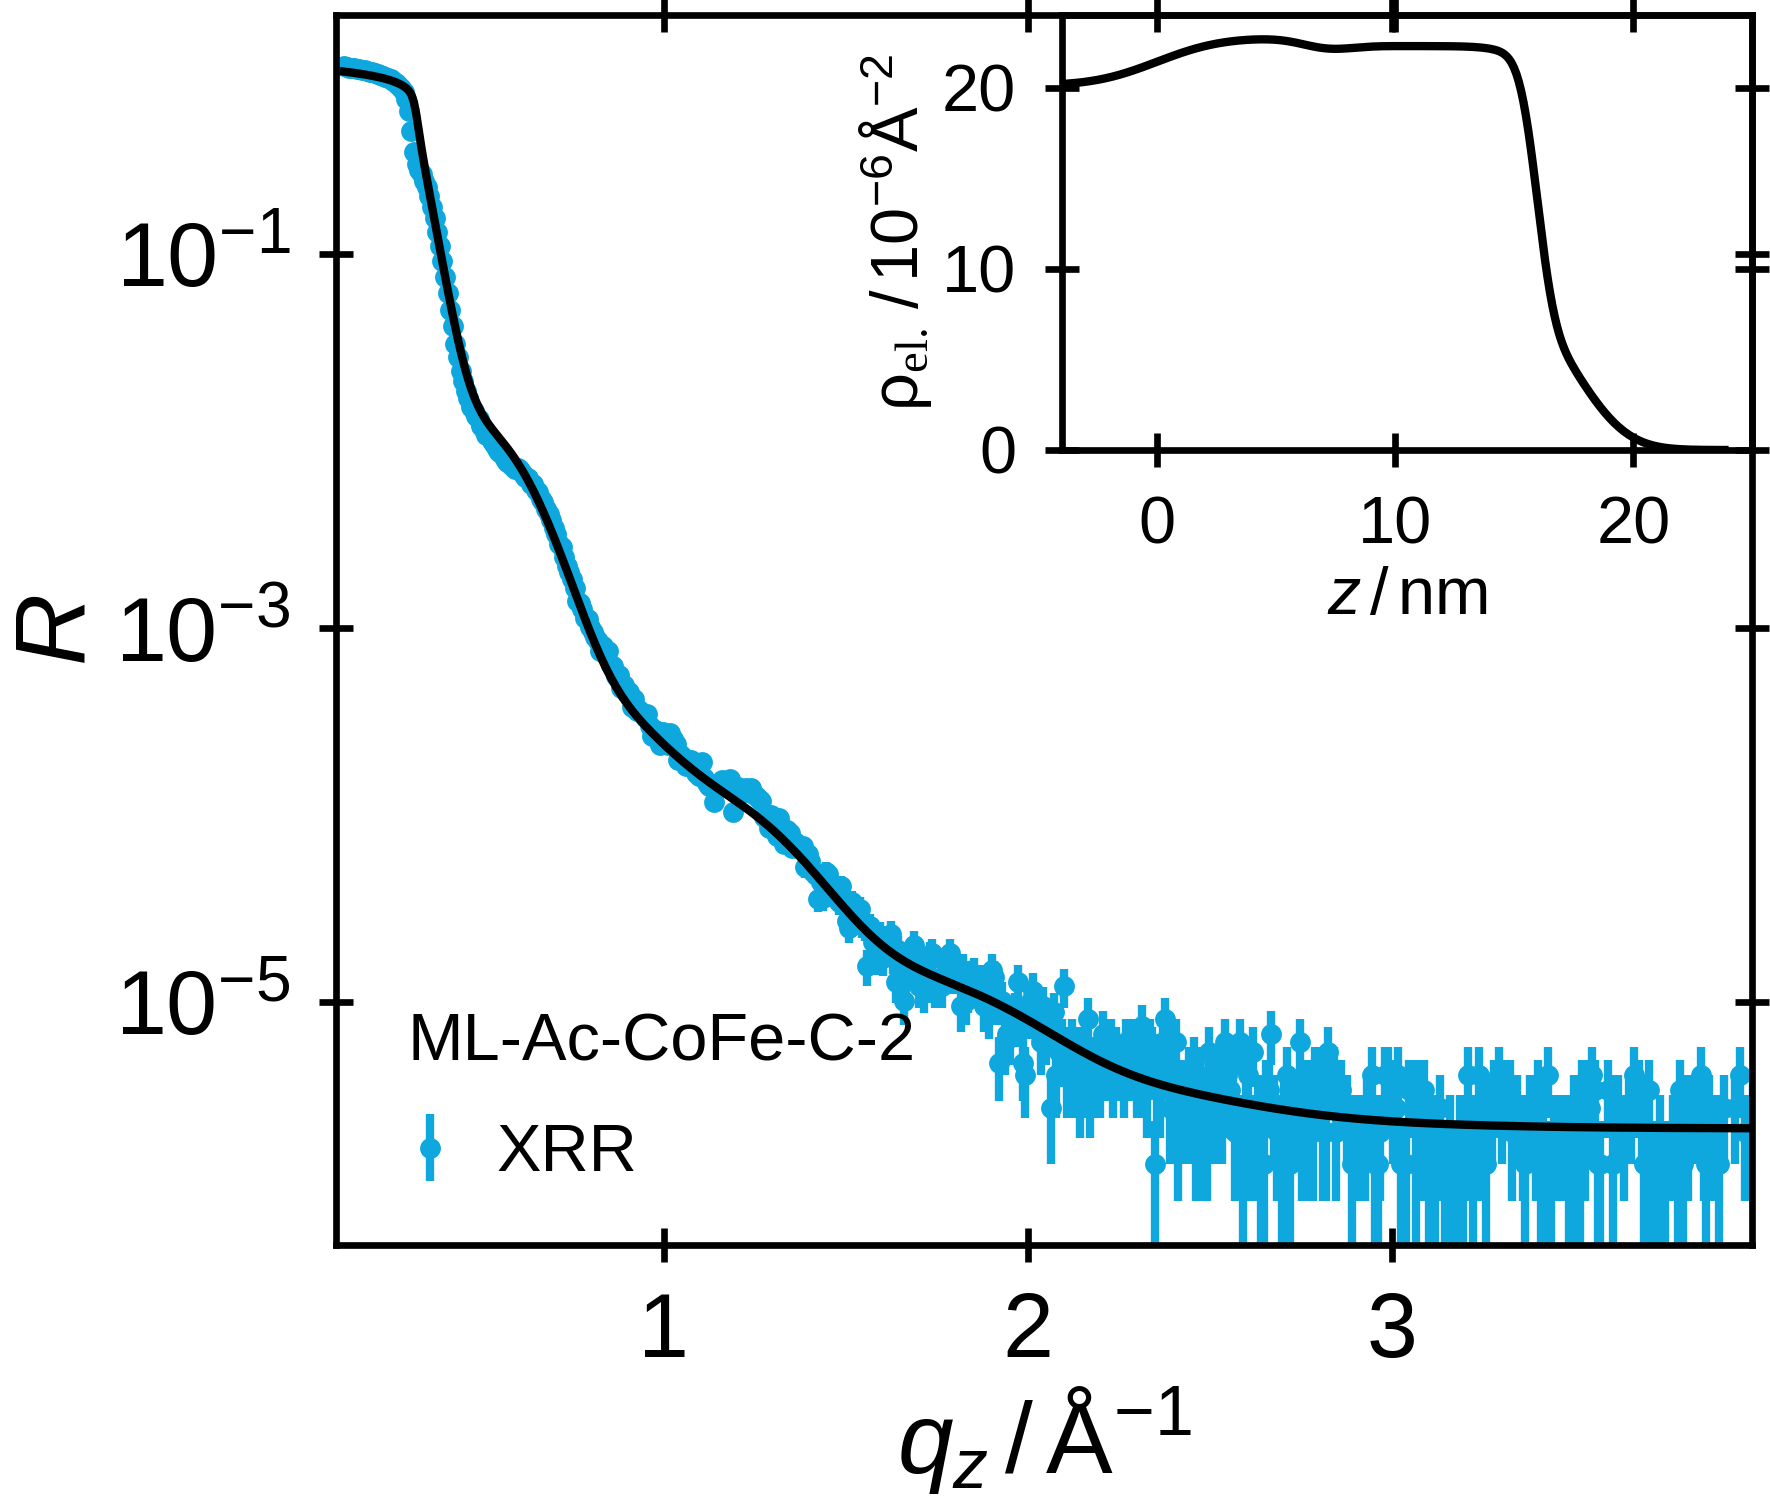
\includegraphics{monolayers_SquareArrayParacrystal_ML_Ac-CoFe-C-2_WithSpacer_XRR}
    \caption{\label{fig:monolayers:structure:squareArrayParacrystal:XRR}XRR of ML-Ac-CoFe-C-2 described according to the model of \refsec{sec:monolayers:structure:verticalModel}.}
  \end{figure}

  In an analogue procedure, ML-Ac-CoFe-C-2 is characterized by XRR, which is shown in \reffig{fig:monolayers:structure:squareArrayParacrystal:XRR}.
  Even though the micrographs of the sample suggest a higher quality monolayer, the reflectivity shows only weakly pronounced peaks.
  Refining the same scattering length density model as used for ML-Ac-CoFe-C, a closely matching reflectivity can be calculated, which is used in the following to discuss and understand the observed reflectivity.

  The refined packing fraction of $53.6(6) \%$ corresponds to a particle spacing of $13.4(2) \unit{nm}$, which is again approximately two oleic acid chain lengths larger than the average nanocube edge length and therefore in a reasonable order of magnitude.
  Inspecting the scattering length density profile, only a weak contrast between the nanocube layer and the silicon dioxide/silicon substrate is observed, which is effectively modeled in the vanishing thickness of the lower oleic acid layer.
  A potential origin for this different observation in comparison to ML-Ac-CoFe-C might be that the silicon dioxide layer has a porous surface, which allows an intermixing of the oleic acid coating of the nanoparticles and therefore the low contrast observed in the SLD profile.
  The weak contrast is then also reason for the observed reflectivity with only low pronounced features.

  \begin{table}[!htbp]
    \centering
    \caption{\label{tab:monolayers:structure:squareArrayParacrystal:XRR}Refined parameters from X-ray reflectometry of ML-Ac-CoFe-C-2 shown in \reffig{fig:monolayers:structure:squareArrayParacrystal:XRR}. The parameter definitions are equivalent to \reftab{tab:monolayers:structure:ML-Ac-CoFe-C-WithSpacer}}
    \begin{tabular}{l | c}
      \hline
      ML-Ac-CoFe-C-2 & \textbf{XRR}\\
      \hline
      $\eta_\mathrm{Cube} \, /\, \%$                  & $53.6(6)$ \\
      $d_{\ch{SiO2}} \, / \unit{nm}$                  & $7.4(8)$ \\
      $d_{\mathrm{OA, lower}}\, / \unit{nm}$          & $0.1(1)$\\
      $d_{\mathrm{OA, upper}}\, / \unit{nm}$          & $1.6(1)$ \\
      $\sigma_{\ch{Si}/\ch{SiO2}} \, / \unit{nm}$     & $1.9(6)$ \\
      $\sigma_{\ch{SiO2}/\mathrm{OA}}\, / \unit{nm}$  & $1.2(2)$ \\
      $\sigma_\mathrm{OA/NC} \, / \unit{nm}$          & $1.1(2)$ \\
      $\sigma_\mathrm{NC/OA} \, / \unit{nm}$          & $0.5(1)$ \\
      $\sigma_\mathrm{OA/air} \, / \unit{nm}$         & $1.4(1)$ \\
      \hline
      $\Delta \lambda / \lambda\, / \unit{\%}$        & $5$ \\
      $I_\mathrm{bg} \, / \unit{10^{-6}}$             & $1.6$\\
      \hline
      $a \, / \unit{nm}$ & $8.58$ \\
      \hline
      $a_\mathrm{p-p} \, / \unit{nm}$ & $13.4(2)$ \\
      \hline
    \end{tabular}
  \end{table}
\end{document}
